\renewcommand{\lsql}[1]{\lstinline[language=SQL,prebreak=]!#1!}

\lab{Python}{Advanced SQL}{SQL II}
\objective{Learn more of the advanced and specialized features of SQL.}
\label{lab:advancedsql}

\section*{Database Normalization}
Normalizing a database is the process of organizing tables and columns to minimize the amount of redundant information in the database.
For example, a non-normalized database might have a table that stores customer contact information and a table that contains all of the products a company has sold.
However, they might want to track who buys what products in case they need to contact them later. To do so, they store all the contact information of a particular buyer along with every item they purchased.
Now, two tables store the customer contact information.
If we needed to update a customer's phone number, we have to update two tables.
While that may not be bad for small databases, larger databases would be near impossible to update correctly.
The idea of normalizing a database allows us to store all customer contact information in one place in the database.
All other tables that might need a customer's name, phone number, or address would reference the contact information table.
When an update needs to be performed, we only need to update the contact information table.
Then any table that references this information is also automatically up to date.

To properly normalize a database, we need to discuss the types of relations tables might have.
\subsection*{One to One}
This is the simplest relation to model.
A single table can be used to express this relation.
The relation is between one record and at most one other record.
An example of this relationship is an employee and their organization.
One employee works at one organization.
Another example would be that a driver's license belongs to only one person.

\subsection*{One to Many}
This relationship and its inverse must be modeled with at least two tables.
The general approach is to use a unique ID.
Note that a relationship that appears one to one may actually be a one to many relationship.
Many people will, therefore, use the same unique ID approach on one to one relationships too in the case it turns out to be a one to many relationship.
An example of a one to many relationship would between an department and its employees.
The department would receive a unique ID and then each employee in that department would be tagged with that ID.

\subsection*{Many to Many}
This relationship requires at least three tables.
A many to many relationship can be visualized as two, separate one to many relationships.
The records in each of the two tables receive a unique ID.
A third table then serves as a map between IDs of table to IDs of the other table.
An example of a many to many relationship is doctors and patients.
One doctor can have several patients and one patient can have several doctors.

For the rest of the lab, we will be using the following tables: \ref{table:students}, \ref{table:majors}, \ref{table:grades}, and \ref{table:classes}.

\begin{table}
\begin{tabular}{|l|l|l|l|}
\hline
StudentID & Name & MajorCode & MinorCode \\
\hline
401767594 & Michelle Fernandez & 1 & NULL \\
678665086 & Gilbert Chapman & NULL & NULL\\
553725811 & Roberta Cook & 2 & 1\\
886308195 & Rene Cross & 3 & 1\\
103066521 & Cameron Kim & 4 & 2\\
821568627 & Mercedes Hall & NULL & 3 \\
206208438 & Kristopher Tran & 2 & 4\\
341324754 & Cassandra Holland & 1 & NULL\\
262019426 & Alfonso Phelps & NULL & NULL\\
622665098 & Sammy Burke & 2 & 3 \\
\hline
\end{tabular}
\caption{students}
\label{table:students}
\end{table}

\begin{table}
\begin{tabular}{|l|l|}
\hline
ID & Name \\
\hline
1 & Math \\
2 & Science \\
3 & Writing \\
4 & Art \\
\hline
\end{tabular}
\caption{fields}
\label{table:majors}
\end{table}

\begin{table}
\begin{tabular}{|l|l|l|}
\hline
StudentID & ClassID & Grade \\
\hline
401767594 & 4 & C \\
401767594 & 3 & B- \\
678665086 & 4 & NULL \\
678665086 & 3 & A+ \\
553725811 & 2 & C \\
678665086 & 1 & NULL \\
886308195 & 1 & A \\
103066521 & 2 & C \\
103066521 & 3 & C- \\
821568627 & 4 & D \\
821568627 & 2 & NULL \\
821568627 & 1 & B \\
206208438 & 2 & A \\
206208438 & 1 & C+ \\
341324754 & 2 & D- \\
341324754 & 1 & NULL \\
103066521 & 4 & A \\
262019426 & 2 & B \\
262019426 & 3 & NULL \\
622665098 & 1 & A \\
622665098 & 2 & A- \\
\hline
\end{tabular}
\caption{grades}
\label{table:grades}
\end{table}

\begin{table}
\begin{tabular}{|l|l|}
\hline
ClassID & Name \\
\hline
1 & Calculus \\
2 & English \\
3 & Pottery \\
4 & History \\
\hline
\end{tabular}
\caption{classes}
\label{table:classes}
\end{table}

\begin{problem}
Classify the relations between the various records in these tables: \ref{table:students}, \ref{table:majors}, \ref{table:grades}, and \ref{table:classes}.

Classify each relation as either one to one, one to many, or many to many.
Identify the tables used in each relationship.
\label{prob:tablerelations}
\end{problem}

\begin{info}
There are instances where you would not want a completely normalized database.
Whether to normalize your database depends on your specific needs.
Usually, though, the decision to denormalize a database is a last-resort attempt to improve performance.
\end{info}

\section*{Joining tables}
We can use SQL to join two or more tables together for a query.
This is a very powerful tool.
SQLite supports three types of standard table joins.

Joining tables is a common practice to collect data from different parts of the database into a single table.
Joins are absolutely essential in a normalized database since data is split between multiple tables.

\subsection*{Inner Join}
This is often the default join operation in SQL.
An inner join can be depicted as an intersection of two or more tables.
\begin{figure}
\centering
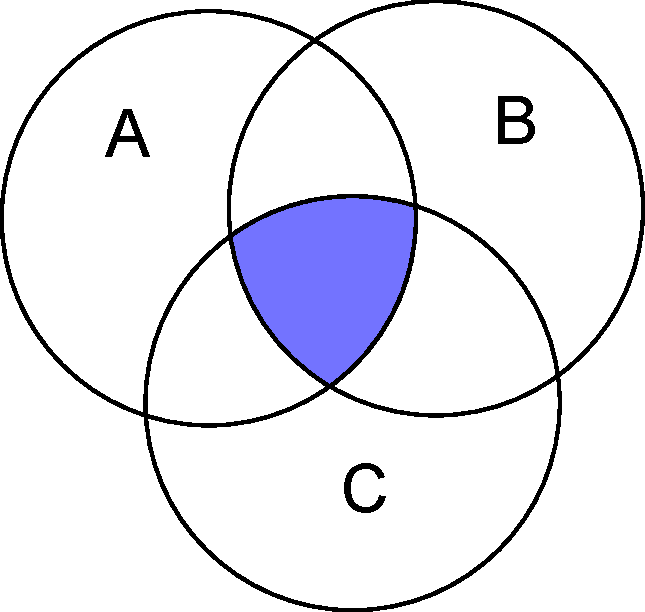
\includegraphics[width=.5\textwidth]{inner_join.pdf}
\caption{An inner joining of tables A, B, and C.}
\label{fig:inner_join}
\end{figure}
When performing an inner join on tables, the result will only be those records that match across all tables.
\begin{lstlisting}[language=SQL]
SELECT students.name, majors.name FROM students JOIN majors ON students.majorcode=majors.id;
\end{lstlisting}
An inner join is equivalent to the following pseudo-loop in Python
\begin{lstlisting}
for row_s in students:
    for row_m in majors:
        if predicates(row_s, row_m):
            yield columns(row_s, row_m)
\end{lstlisting}

\begin{table}
\begin{tabular}{|l|l|}
\hline
students.name & majors.name \\
\hline
Michelle Fernandez & Math \\
Roberta Cook & Science \\
Rene Cross & Writing \\
Cameron Kim & Art \\
Kristopher Tran & Science \\
Cassandra Holland & Math \\
Sammy Burke & Science \\
\hline
\end{tabular}
\caption{An inner join of students and majors}
\label{table:ij_studentsmajors}
\end{table}

\subsection*{Left Outer Join}
A left outer join will return all relations from the left table even if they don't match any relation on the joined tables.
An illustration of a left outer join is given in figure \ref{fig:left_outer}.
\begin{figure}
\centering
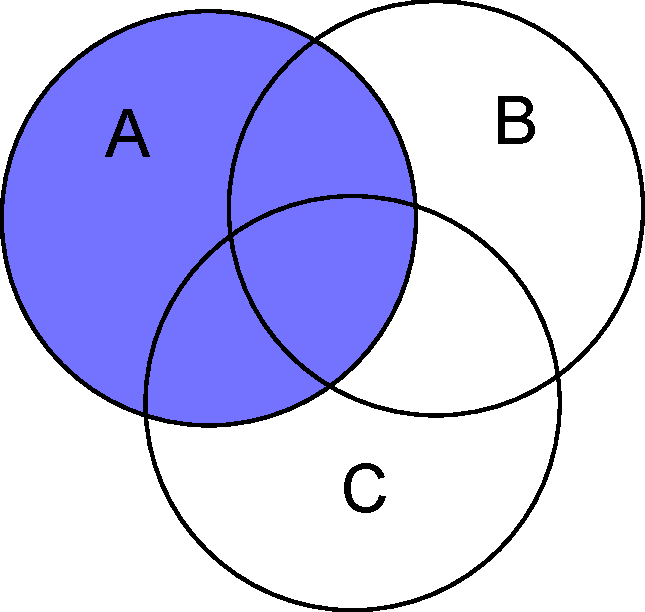
\includegraphics[width=.5\textwidth]{left_outer.pdf}
\caption{A left outer table join of A with tables B and C.}
\label{fig:left_outer}
\end{figure}

A Pythonesque loop that illustrates performs a left outer join is
\begin{lstlisting}
for row_s in students:
    for row_m in majors:
        if predicates(row_s, row_m):
            yield columns(row_s, row_m)
        else:
            yield columns(row_s)
\end{lstlisting}

The following left outer join will result in the table shown in table \ref{table:lo_studentsmajors}.
\begin{lstlisting}[language=SQL]
SELECT students.name, majors.name FROM students LEFT OUTER JOIN majors ON students.majorcode=majors.id;
\end{lstlisting}
\begin{table}
\begin{tabular}{|l|l|}
\hline
students.name & majors.name \\
\hline
Michelle Fernandez & Math \\
Gilbert Chapman & None \\
Roberta Cook & Science \\
Rene Cross & Writing \\
Cameron Kim & Art \\
Mercedes Hall & None \\
Kristopher Tran & Science \\
Cassandra Holland & Math \\
Alfonso Phelps & None \\
Sammy Burke & Science \\
\hline
\end{tabular}
\caption{A left outer join of students and majors}
\label{table:lo_studentsmajors}
\end{table}

\subsection*{Cross Join}
Essentially a Cartesian product of tables.  
Care must be taken when using cross join because of the size of the joined table.
A cross join should only be used on small tables.
It matches each relation in one table with every other possible combination of relations in the joined tables.

\section*{Advanced Selections}
Aggregate functions are useful for summarizing the data in a column.
The functions are
\begin{table}
\begin{tabular}{|l|l|}
\hline
Function & Description \\
\hline
MIN() & Retrieve the smallest numeric value of a column \\
MAX()& Retrieve the largest numeric value of a column \\
SUM() & Sum the numeric values of a column \\
AVG() & Retrieve the average numeric value of the column \\
COUNT() & Retrieve the total number of matching records in a column \\
\hline
\end{tabular}
\label{table:aggregations}
\caption{SQL aggregation functions}
\end{table}

We can count the number of students by executing the following SQL statement.
\begin{lstlisting}[language=SQL]
SELECT COUNT(*) FROM students;
\end{lstlisting}

\subsection*{Ordering and Grouping Relations}
The \lsql{ORDER BY} keyword can be used to sort the result set by columns.
We can sort in ascending order or descending order.
\begin{lstlisting}[language=SQL]
SELECT name FROM students ORDER BY name ASC;
SELECT name FROM students ORDER BY name DESC;
\end{lstlisting}

Another useful SQL keyword is the \lsql{GROUP BY} keyword.
It is used along with an aggregating function to group the result set by columns.
\begin{lstlisting}
SELECT grade, COUNT(studentid) FROM grades GROUP BY grade;
\end{lstlisting}
The result set is given in table \ref{table:group_by_grade}.
\begin{table}
\begin{tabular}{|l|l|}
\hline
grade & COUNT(studentid) \\
\hline
None & 5 \\
A & 4 \\
A+ & 1 \\
A- & 1 \\
B & 2 \\
B- & 1 \\
C & 3 \\
C+ & 1 \\
C- & 1 \\
D & 1 \\
D- & 1 \\
\hline
\end{tabular}
\caption{Grouping of students by grade.}
\label{table:group_by_grade}
\end{table}

\begin{problem}
Write a SQL query that will count how many students belong to each major, including students that don't have a major.  Sort your results in ascending order by name.
Your result set should be table \ref{table:grouporder}
\begin{table}[H]
\begin{tabular}{|l|l|}
\hline
None & 3 \\
Art & 1 \\
Math & 2 \\
Science & 3 \\
Writing & 1 \\
\hline
\end{tabular}
\caption{Result set}
\label{table:grouporder}
\end{table}
\label{prob:studentmajors}
\end{problem}

Another important keyword is the \lsql{HAVING} keyword.
This is necessary because the \lsql{WHERE} clause does not support aggregate functions.
A \lsql{HAVING} clause requires a \lsql{GROUP BY} clause.
The following will not work.
\begin{lstlisting}[language=SQL]
SELECT grade FROM grades GROUP BY grade WHERE COUNT(*)=1;
\end{lstlisting}
Since \lsql{COUNT} is an aggregating function, the following is required.
\begin{lstlisting}[language=SQL]
SELECT grade FROM grades GROUP BY grade HAVING COUNT(*)=1;
\end{lstlisting}
This SQL query returns all the grades that occur only once in the table.
A simple why to remember the difference is \emph{\lsql{WHERE} operates on individual records and \lsql{HAVING} operates on groups of records}.

\begin{problem}
Select all the students who have received grades (non-null grades) in more than two classes.  How many grades did he receive?
\label{prob:manygrades}
\end{problem}

\subsection*{Case Expression}
A case expression allows you to temporarily modify records from a select operation.
There are two forms of the case expression; simple and searched.
The simple form of the expression is a match and replace on a specified column.
A simple case expression is demonstrated below.
\begin{lstlisting}[language=SQL]
SELECT name, 
CASE majorcode 
    WHEN 1 THEN 'Math' 
    WHEN 2 THEN 'Science' 
    WHEN 3 THEN 'Writing' 
    WHEN 4 THEN 'Art' 
    ELSE 'Undeclared' 
    END AS major
FROM students;
\end{lstlisting}

A searched case expression using a boolean expression for the \lsql{WHEN} clauses.
\begin{lstlisting}[language=SQL]
SELECT name, 
CASE 
    WHEN majorcode IS NULL THEN 'Undeclared' 
    ELSE majorcode 
    END AS major, 
CASE 
    WHEN minorcode IS NULL THEN 'Undeclared' 
    ELSE minorcode 
    END AS minor 
FROM students;
\end{lstlisting}

\begin{problem}
Find the overall GPA of all the students in the school.
Use a regular 4.0 scale (A=4.0, B=3.0, C=2.0, D=1.0).
Any pluses or minuses are dropped so an A- becomes and A.

Your result set should be one column and one row with average of all GPAs of all the students taking classes.  
Your solution should return a single floating point number.

Use the \lsql{ROUND()} function in SQL to round your result to the nearest hundredth.
\label{prob:studentGPA}
\end{problem}

\begin{problem}
The SQL keyword, \lsql{LIKE}, allows us to match patterns in a column.
For example,
\begin{lstlisting}[language=SQL]
SELECT name, studentid FROM students WHERE studentid LIKE '\%4';
\end{lstlisting}
will return all the students that have a student ID that ends with the digit 4.

Write a SQL statement that will find all students with a last name that begins with the letter `C' and return their names and majors.  Your returned records should be
\begin{table}[H]
\begin{tabular}{|l|l|}
\hline
Gilbert Chapman & None \\
Roberta Cook & Science \\
Rene Cross & Writing \\
\hline
\end{tabular}
\label{table:likec_solution}
\end{table}
\label{prob:likec}
\end{problem}

\let\undefined\lsql 
